The rocket landing control problem is challenging, containing a high-dimensional observation and action space, along with dynamic uncertainties from the atmosphere and complex non-linear rocket dynamics, for instance, from fuel sloshing. At the same time, it needs to be safety-critical; as a result, a robust and adaptive solution must be used to compensate for the disturbances and uncertainties.

Current control methods for rocketry use loss-less convexification with SOCP solvers or an MPC to control for the trajectory which can take significant computational resources. Linear Quadratic Regulators (LQR), Proportional-Integral Derivative controllers (PID) and feed-forward models are traditional method for attitude and motion control, with proven theory allowing for stability and robustness metrics. This thesis aims to study the feasibility of using a data-driven strategy instead of currently used methods.

This is motivated by recent studies into RL applications highlighting data-driven controllers as a promising alternative to work well within the problem definition. As optimal control can be learnt through policies gained by interacting with a simulation environment without the need for complex mathematics or optimisation solvers. Secondly, they can constructed in a way to allow for robust and adaptive control. Finally, if as they are realisable they require less computational time in real-time scenairos than traditional trajectory optimisation methods.

Data-driven methods have been divided into groups focused around four main features, as presented in \autoref{fig:data_driven_family_tree}.
\begin{itemize}
    \item The learning strategy (\autoref{sec:line}) chooses whether learning will occur on of offline, determining whether they update within flight or train on a fixed dataset.
    \item Policy learning (\autoref{sec:policy}) decides to use off or on policy learning, referring whether to update the policy experiences generated by the current policy.
    \item The control has the option to use a model to guide decision making through model-based methods. Alternatively, model-free methods learn a policy through learn policies through environment interaction without use a learnt model to change its policy. \autoref{sec:model_methods} covers this.
    \item The algorithm family (\autoref{sec:TD_MC_DP_ES}) causes the best data-driven learning algorithm for the study.
\end{itemize}

\begin{figure}[H]
    \centering
    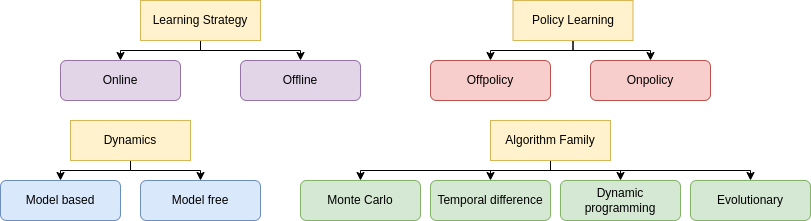
\includegraphics[width=0.85\linewidth]{figures/LiteratureStudy/DataDriven_familytree.png}
    \caption{Data driven methods family tree}
    \label{fig:data_driven_family_tree}
\end{figure}


\subsection{Online vs Offline learning}
\label{sec:line}

Policy learning can be divided into online and offline learning (\cite{sutton1998reinforcement}). Offline learning uses pre-collected data/simulations to train policies, while online learning can dynamically adapt to the environment in real time.

Offline learning allows for training before deployment, which is practical in safety-critical applications like rocket landings. As rocket landings are expensive and highly risky, it is important to learn extensively in a simulation beforehand. Online learning would allow a rocket to adapt during flight to disturbances and dynamic environments arising from the atmosphere and the complex non-linear dynamics of rocketry. However, it can lead to unpredictability and an increased computational overhead.

\textbf{Online learning}, within simulations, is chosen as the policy the rocket initially has will not be sufficient for landing. Resulting, in an updating policy needed to unlock new a better experiences bringing to a feasible landing before optimisation can occur.

\subsection{Off-policy vs On-policy methods}
\label{sec:policy}

The off/on policy decision determines how agents use their environment transitions to learn optimal policies (\cite{sutton1998reinforcement}). On-policy algorithms determine and improve the current policy executed by the agent, for instance, in SARSA, where the action-value function is updated by the agent for each action taken. Off-policy methods learn the optimal policy independently from the current actions taken during exploration; for instance, Q-learning updates the action-value function through the expected maximum cumulative rewards of future actions.

\textbf{Off-policy} methods are more sample efficient as they can reuse previous transitions through a buffer and as such is chosen. Also, in a stochastic environment, the policy updated takes into account transitions from other episodes which had different disturbances.

\subsection{Model-free vs Model-based methods}
\label{sec:model_methods}

\textbf{Model-free} control methods are well-suited for a rocket landing control system as they learn optimal policies without relying on a high-fidelity mathematical model of the dynamics and disturbances. High-fidelity models require an accurate knowledge of the non-linear and complex dynamics, which is infeasible to make by one person. Secondly, model-free methods can allow environmental exploration to adapt to uncertainties and disturbances, making them robust and adaptive. If the model-free algorithm can transfer well to higher-fidelity models, it shows a proof of concept for using data-driven control for rocket landing. Furthermore, \cite{Jiang2024} used an RL framework with "random annealing jump start" to jump-start learning and improved success rates through a model-free algorithm. Offering an indication of the initial feasibility of this project.

\subsection{Algorithm families}
\label{sec:TD_MC_DP_ES}

The rocket landing control problem has a continuous, high-dimensional state, observation and action spaces, and complex, uncertain, non-linear dynamics. \textbf{Temporal Difference} (TD), like Q-learning and State-Action-Reward-State-Action (SARSA), uses incremental learning to update value estimates from differences in actual and predicted rewards (\cite{sutton1998reinforcement}). Combining with neural networks to act as function approximators, it can effectively handle complex and continuous problems (\cite{mnih2013playing}) while being model-free.

In contrast, Dynamic Programming (DP) need full knowledge of the environment; while extensions to the method can leverage neural networks for this, it is often impractical for large systems due to the high computation requirements (\cite{cmu2021recitation}). Monte Carlo methods (\cite{sutton1998reinforcement}) average returns over complete episodes, making them less efficient for tasks like rocket landing, where long episodes may occur. Evolutionary methods optimise policies without using gradients and are parallelisable; however, they can be sample-inefficient due to a large number of policies being ran to cover the search space. As such, TD methods are chosen as they seem the most relevant to the problem.